\section{Álgebra Geométrica Conforme}
En la sección pasada se describió la estimación de los modelos usando RANSAC. En esta sección se presentan modelos matemáticos para el plano, esfera y cilindro en AGC y las funciones usadas para validar los puntos del modelo.\\

Las entidades en AGC cuentan con dos representaciones (IPNS y OPNS), ya que es fácil pasar de una forma a otra se puede trabajar con cualquiera de ellas dependiendo de las necesidades.\\

Una \gls{esfera} en AGC en IPNS se representa como se observa en la ecuación \eqref[ec.]{eq:esferaAGC1}, donde $P$ es el centro en AGC y $r$ el radio de la esfera, y en OPNS como la ecuación \eqref[ec.]{eq:esferaAGC2}, donde $P_i$ son puntos de AGC que se encuentran en la superficie de la esfera.

\begin{equation}
    \label{eq:esferaAGC1}
    S=P-\frac{1}{2}r^2 e_\infty
\end{equation}

\begin{equation}
    \label{eq:esferaAGC2}
    S^\ast=P_1\land P_2\land P_3\land P_4
\end{equation}

Ya que para el algoritmo de RANSAC hay que crear un modelo, esto se realiza de forma similar que para una esfera AE usando cuatro puntos. lo único que falta para crear el modelo es escribir un punto de AE en AGC para eso se usa la ecuación \eqref[ec.]{eq:puntoAGC}, donde $\mathbf{x}$ es el vector $(x,y,z)$.

\begin{equation}
    \label{eq:puntoAGC}
    P={\mathbf{x}}+\frac{1}{2}\mathbf{x}^2e_\infty+e_0
\end{equation}
La forma de validar si un punto se encuentra sobre la superficie de la esfera es diferente al usado en AE ya que no hay forma directa para calcular la distancia más corta, sin embargo, es posible calcular la distancia del punto a la tangente de la esfera como se muestra en la figura \ref{fig:ps} usando la ecuación \eqref[ec.]{eq:ps1}, donde $s$ es el vector $(S_1,S_2,S_3)$ y $p$ es el vector $(P_1,P_2,P_3)$ \cite{FoundOfAGC}.

\begin{figure}[!htb]
    \centering
    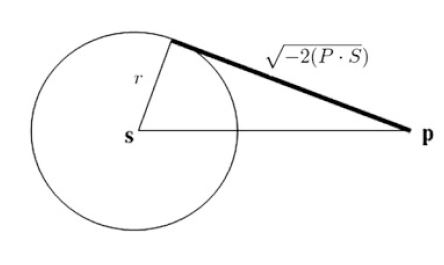
\includegraphics[width=0.6\textwidth]{02Desarrollo/AGC/imagenes/distPtoS.JPG}
    \caption[Distancia entre un punto y una esfera.]{El producto interno de un punto y una esfera describe el cuadrado de la distancia entre el punto y la tangente de la esfera.}%\cite{FoundOfAGC}} 
    \label{fig:ps}
\end{figure}
            
\begin{equation}
    \label{eq:ps1}
    P\cdot S=\frac{1}{2}r^2 -\frac{1}{2} (s-p)^2
\end{equation}

De tal manera que la distancia $\sqrt{-2(P\cdot S)}$ entre el punto y el punto tangente a la esfera esta dado por la ecuación \eqref[ec.]{eq:ps2}
\begin{equation}
    \label{eq:ps2}
    -2(P\cdot S)=(s-p)^2 - r^2
\end{equation}

Para encontrar el modelo del \gls{plano}, se realiza de manera similar a la esfera, primero hay que convertir los puntos usando la ecuación \eqref[ec.]{eq:puntoAGC}, y usar la representación de un plano en forma OPNS que se muestra en la ecuación \eqref[ec.]{eq:planeAGC2}, donde $P_i$ son puntos en la superficie del plano, y la forma IPNS está dada por la ecuación \eqref[ec.]{eq:planeAGC1}, donde $\mathbf{n}$ es el vector normal del plano y $d$ la distancia del origen al plano sobre el vector normal $n$.
\begin{equation}
    \label{eq:planeAGC2}
    \pi^\ast=P_1\land P_2\land P_3\land e_\infty
\end{equation}
\begin{equation}
    \label{eq:planeAGC1}
    \pi={\mathbf{n}}+de_\infty
\end{equation}

Determinar si los puntos se encuentran dentro de la superficie del plano, se usa la ecuación \eqref[ec.]{eq:ppi} que determina la distancia entre el punto y el plano, donde $\pi^\ast$ es el plano en la forma OPNS, $P$ es el punto en AGC, $p$ es el vector $(x,y,x)$ de $P$, $n$ es el vector normal al plano y $d$ la distancia del origen al plano.

\begin{equation}
    \label{eq:ppi}
    P\cdot \pi^\ast=p\cdot n-d
\end{equation}

 Para la creación del \gls{cilindro} es un poco más compleja, ya que no se cuenta con una identidad para crear el cilindro es necesario construirlo usando el modelo creado a partir de dos esferas descrito por Aksel Sveier \cite{cilindrosAGC}. \\
 
 El cilindro se crea con un eje y un radio, para encontrar el eje se buscan dos esferas usando el método RANSAC y trazando una línea entre sus centros se obtiene el eje del cilindro, como se muestra en la figura \ref{fig:05AntecedentesB}, para obtener el radio del cilindro se promedian los radios de las esferas.\\
 
 La construcción de una línea que pasa por el centro de dos esferas se calcula usando la ecuación \eqref[ec.]{eq:lineaAGC}, donde $S_i^\ast$ es una esfera en la forma OPNS.
 \begin{equation}
     \label{eq:lineaAGC}
     L=S_1^\ast \land S_2^\ast \land e_\infty
 \end{equation}
 
 La forma de saber si un punto pertenece al cilindro es creando una esfera cuyo centro pasa por el eje del cilindro y el ecuador de la esfera pasa por el punto a evaluar, si el radio de la esfera coincide con el radio del cilindro el punto pertenece al cilindro.\\
 
La construcción de la esfera necesaria para conocer si un punto pertenece a un cilindro está dada por la ecuación \eqref[ec.]{eq:cp}, donde $P$ es el punto en AGC a evaluar, $L^\ast$ es la línea que pasa por el eje del cilindro.

\begin{equation}
    \label{eq:cp}
    S_1=\frac{P \land L^\ast}{L^\ast}
\end{equation}

Para obtener el radio $r$ de una esfera en AGC se usa el producto interno de la esfera por sí misma, como se muestra en la ecuación \eqref[ec.]{eq:resf}.
\begin{equation}
    \label{eq:resf}
    r=\sqrt{S_1\cdot S_1}
\end{equation}

\subsection{Herramientas para el uso del AGC}
	
	Para la experimentación con el AGC existen una variedad de herramientas listadas a continuación:
	\begin{itemize}
		\item Cinderella \cite{Cinderel45:online}
		\item GAViewer \cite{Geometri75:online}
		\item CluCalc/CluViz \cite{CLUCalc12:online}
		\item Gaalop \cite{GaalopGe19:online}
		\item Versor \cite{versor}
		\item Versor.js \cite{versorJswe94:online}
	\end{itemize}
	
	Se uso la herramienta GAViewer como se muestra en la figura \ref{fig:GAViwer} para experimentar y validar operaciones en AGC. GAViewer es un programa multipropósito para el computo de operaciones en AG creado por Daniel Fontijne, Leo Dorst, Tim Bouma de la universidad de Ámsterdam y Stephen Mann de la universidad de Waterloo, cuenta con una interfaz gráfica y entrada por comandos en los cuales se pueden trabajar con diferentes AG, así como AGC, permite la conexión de otros programas para realizar las operaciones de AG y visualizar los resultados. El uso de este programa para un desarrollo robusto es limitado ya que el lenguaje de programación usado es lento y con limitaciones\cite{Geometri75:online}.\\
	
	\begin{figure}[!htb]
		\centering
		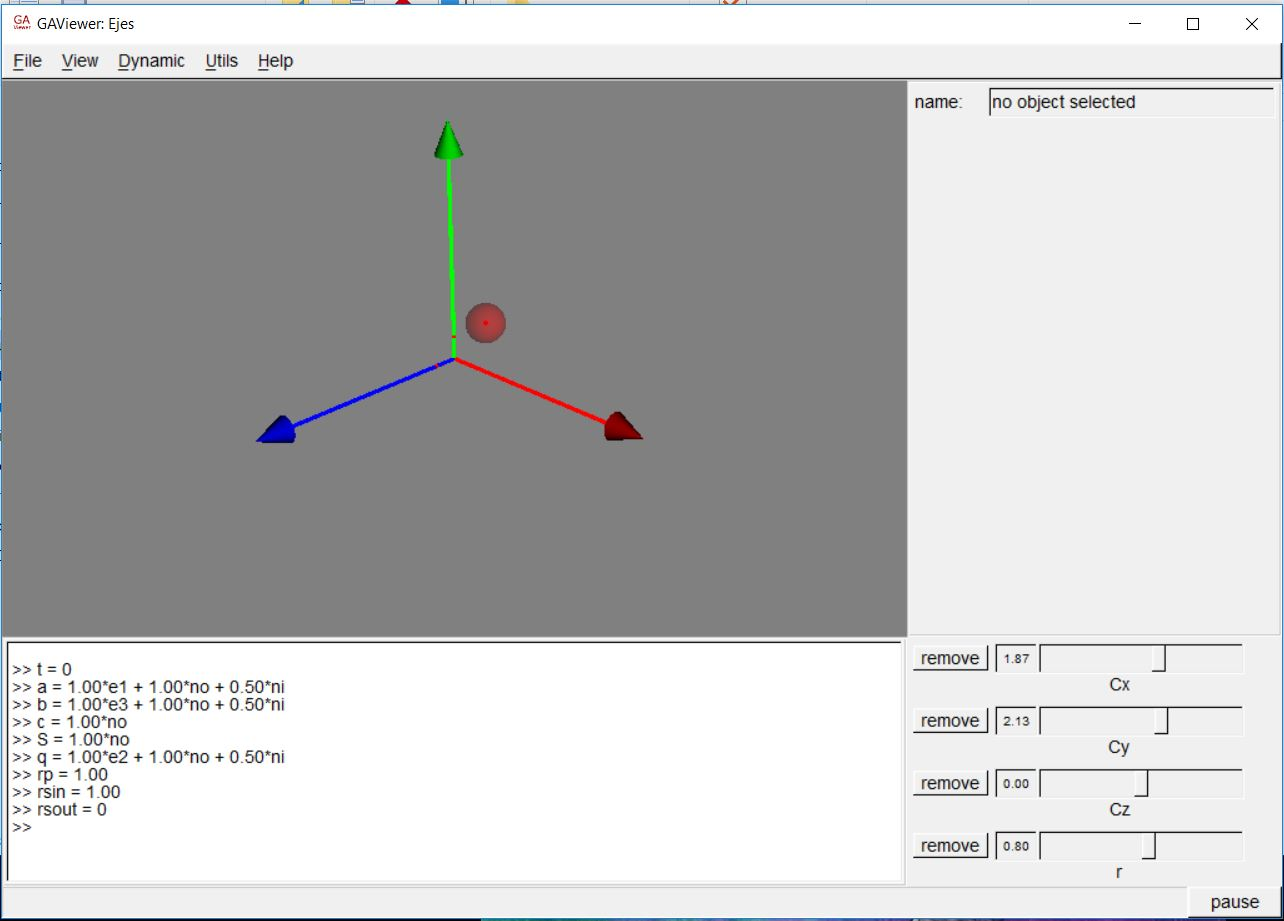
\includegraphics[width=0.9\textwidth]{02Desarrollo/AGC/imagenes/GAViewer.JPG}
		\caption{Programa GAViewer}%\cite{FoundOfAGC}} 
		\label{fig:GAViwer}
	\end{figure}
	

	Para el desarrollo del sistema se usó la biblioteca Versor \cite{versor}, el cual cuenta con soporte para AG, AE, AGC, entre otros tipos de álgebras, permite modificar y acoplar las funciones al sistema y evitar tener que establecer conexiones con otros programas como con el caso de GAViewer. La biblioteca cuenta con funciones matemáticas, así como funciones para la creación de gráficos usando OpenGL y OpenGL ES\\
	
